\begin{frame} % Focus
\frametitle{Focus}
\centering
\textbf{Which mobile robots can meet these requirements?}
\end{frame}

\begin{frame} % 相关工作(腿式)
\frametitle{Related Work}
\begin{columns}
\column{0.5\textwidth}
\textbf{Legged mobile robots:}

\begin{itemize}
    \item Advantages
    \begin{itemize}
        \item Suitable for uneven terrain
        \item Agile mobility
    \end{itemize}
    \item Disadvantages
    \begin{itemize}
        \item Weak load capacity
        \item High power
        \item Unable to turn flexibly
    \end{itemize}
\end{itemize}

\column{0.5\textwidth}
\begin{figure}
    \centering
    \vspace{-1.2cm}
    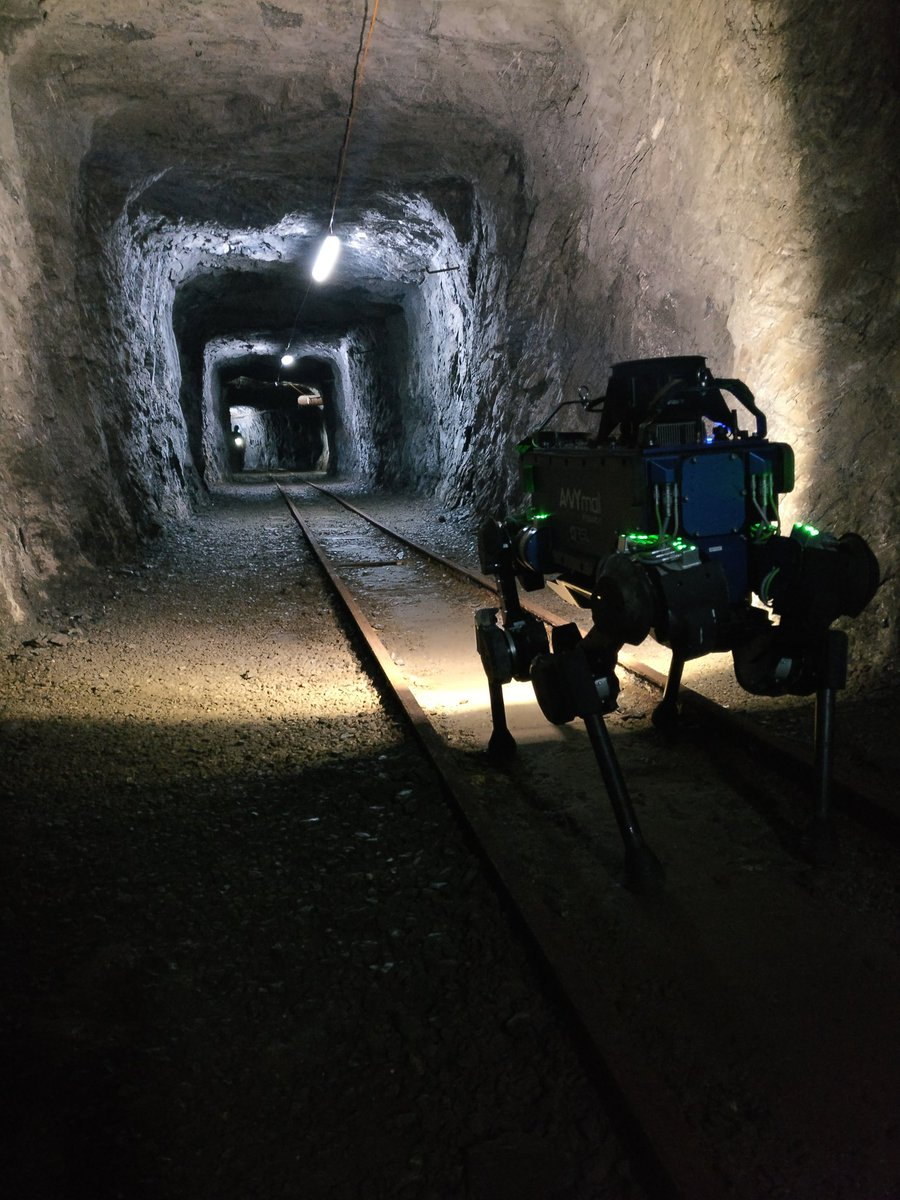
\includegraphics[width=4.5cm]{photos/qua-leg.png} 
    \vspace{-0.3cm}
    \caption{Anymal in Sub-T Challenge}
    \label{fig:sub-t}
    \vspace{-0.7cm}
\end{figure}
\end{columns}
\end{frame}

\begin{frame} % 相关工作(轮式)
\frametitle{Related Work}
\begin{columns}
\column{0.5\textwidth}
\textbf{Wheeled omni-directional mobile robots:}

\begin{itemize}
    \item Advantages
    \begin{itemize}
        \item Strong load capacity
        \item Agile omni-directional mobility
    \end{itemize}
    \item Disadvantages
    \begin{itemize}
        \item Not feasible for outdoor usage (Mecanum)
        \item Unable to steer rapidly (4WS-4WD)
    \end{itemize}
\end{itemize}

\column{0.5\textwidth}
\begin{figure}
    \centering
    \vspace{-1.2cm}
    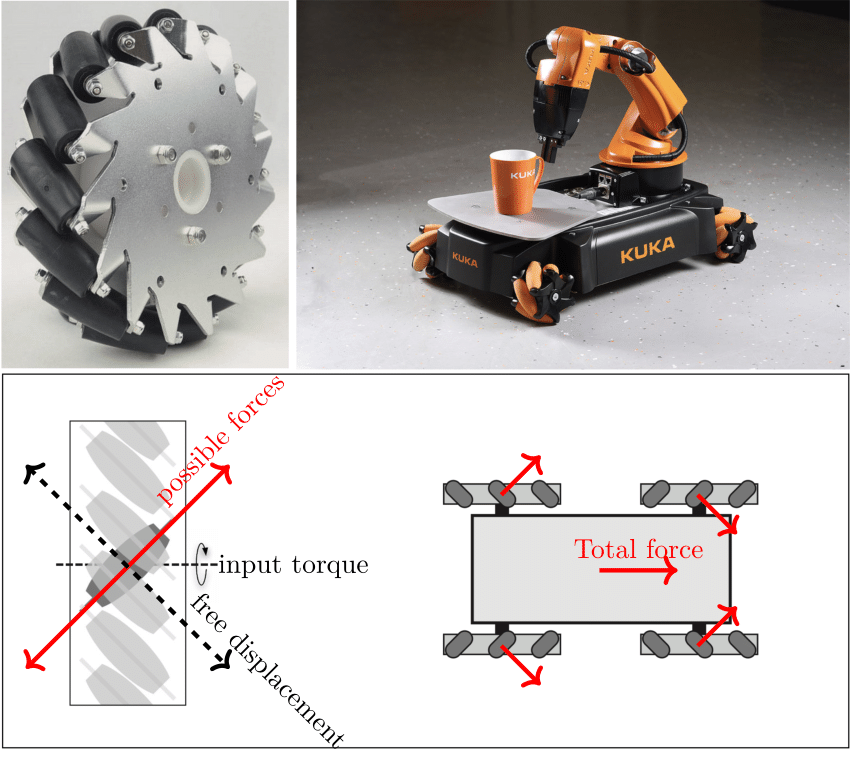
\includegraphics[width=4cm]{photos/mecanum.png} 
    \vspace{-0.3cm}
    \caption{Youbot from KUKA}
    \label{fig:Macanum}
    \vspace{-0.7cm}
\end{figure}

\begin{figure}
    \centering
    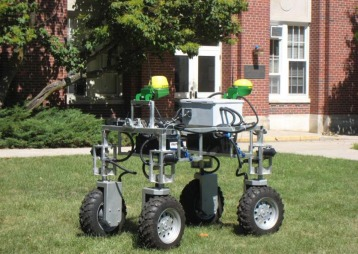
\includegraphics[width=4cm]{photos/4WS-4Wd.png} 
    \vspace{-0.3cm}
    \caption{4WS-4WD robot}
    \label{fig:4ws-4wd}
    \vspace{-0.7cm}
\end{figure}
\end{columns}
\end{frame}

\begin{frame} % 相关工作(轮腿混合)
% 轮式与足式的融合交叉发展 
% 腿-》轮   轮-》腿
\frametitle{Related Work}
\begin{columns}
\column{0.4\textwidth}
\textbf{Wheel-legged mobile robots:}

\begin{itemize}
    \item Developed from wheeled robot: 
    \begin{itemize} 
        \item Add active joints to the body
    \end{itemize} 
    \item Developed from legged robot: 
    \begin{itemize} 
        \item Add wheels on joints
    \end{itemize} 
\end{itemize} 


\textbf{Robots still have some disadvantages!}

\column{0.55\textwidth}
\begin{figure}
    \centering
    \vspace{-1.2cm}
    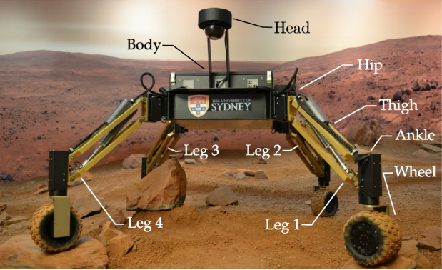
\includegraphics[width=4cm]{photos/wheel-leg.png} 
    \vspace{-0.3cm}
    \caption{Wheel-on-Leg Rover from KUYD}
    \label{fig:wheel-leg}
    \vspace{-0.3cm}
\end{figure}

\begin{figure}
    \centering
    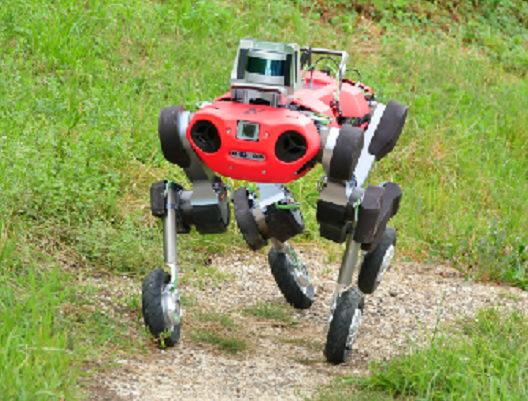
\includegraphics[width=4cm]{photos/anymal-1.png} 
    \vspace{-0.3cm}
    \caption{wheeled quadruped from ETH}
    \label{fig:anymal-1}
    \vspace{-0.7cm}
\end{figure}
\end{columns}
\end{frame}

